\documentclass[a4paper,12pt]{article}

\usepackage{geometry}
 \geometry{
 a4paper,
 lmargin=20mm,
 tmargin=20mm,
 rmargin=20mm,
 bmargin=20mm,
 }

\usepackage[utf8]{inputenc}
\usepackage[english,russian]{babel}

\usepackage{graphicx}
\graphicspath{ {images/} }

\usepackage{csquotes}
\usepackage[
    style=gost-authoryear-min,
    movenames=false
]{biblatex}
\addbibresource{citations.bib}

\usepackage[russian]{cleveref}

\title{Автоматизированный бенчмаркинг алгоритмов решения CVRP}
\author{Андрей Прохоров}
\date{\vspace{-5ex}}
%\date{}  % Toggle commenting to test

\begin{document}

\maketitle

\section*{Почему CVRP}

CVRP - это один из базовых вариантов задачи маршрутизации, который подразумевает наличие одного склада, множества клиентов и транспортных средств.
Задача заключается в создании таких маршрутов для транспортных средств, общая длина которых будет минимальной (\cref{img_cvrp_example}).

\begin{figure}[h]
    \centering
    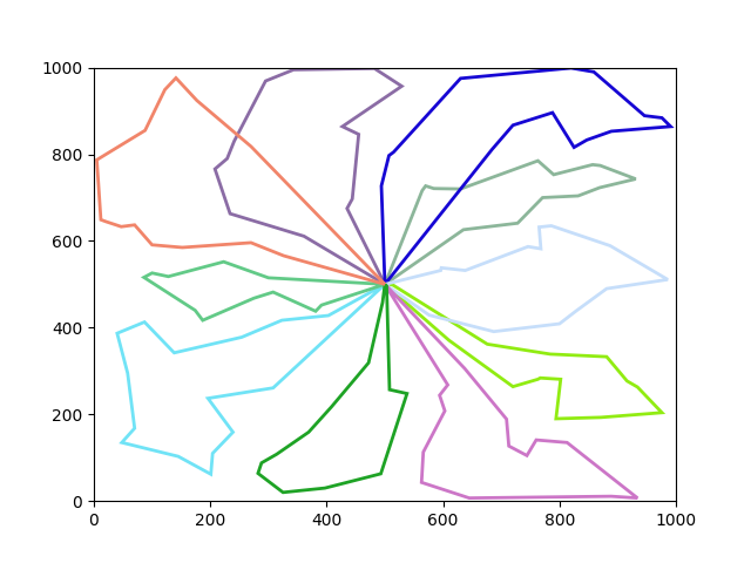
\includegraphics[
        width=0.7\textwidth
    ]{images/cvrp_example.png}
    \caption{
        Решение задачи из набора X
        \autocite{uchoaNewBenchmarkInstances2017}
        алгоритмом HGS
        \autocite{vidalHybridGeneticSearch2022}.
    }
    \label{img_cvrp_example} 
\end{figure}

Эта задача принадлежит к классу \emph{NP-сложных}, и её точное решение на больших входных данных заняло бы  непрактично долгое время.
Поэтому исследователи создают примерные способы её решения, \emph{эвристики}, и используют уже существующие для других задач эвристики, \emph{метаэвристики}.

CVRP продолжает быть популярной среди исследователей и только с 2019 года с её упоминанием было выпущено \emph{5980 статей}, индексируемых в \emph{Google Scholar}.

Также постоянно изобретаются новые эвристики, решающие эту задачу.
Однако всё ещё не существует консенсуса о методах сравнения этих решений. Каждый исследователь сравнивает свой метод с известными произвольным образом, что может повлиять на достоверность таких сравнений.

\section*{Решение}
Для решения этой проблемы я разрабатываю универсальный инструмент бенчмаркинга алгоритмов решения CVRP, который сравнивает среднюю производительность методов по каждой из задач набора бенчмарков к единому моменту времени.
То есть, все алгоритмы останавливают свою работу после достижения момента времени $T$.

Для достижения достоверности сравнения предварительно автоматически выбираются оптимальные гиперпараметры для каждого из алгоритмов.

На данном этапе решение представляет собой библиотеку для языка Python.
В функционал библиотеки также входит возможность запуска на суперкомпьютерах.

\section*{Тестирование решения}
Для проверки работоспособности библиотеки и эффективности предложенного метода требуется испытание на ней нескольких различных алгоритмов решения CVRP при разных условиях, чтобы изучить зависимость результатов сравнения от них:

\begin{enumerate}
    \item При разных ограничениях по времени исполнения $T$;
    \item При разных вычислительных мощностях;
    \item При разном количестве итераций на:
    \begin{itemize}
        \item поиск гиперпараметров;
        \item бенчмаркинг;
    \end{itemize}
    \item[] И при других \dots
\end{enumerate}

Для выполнения таких вычислений на нескольких алгоритмах на 100 задачах с несколькими десятками итераций как для поиска гиперпараметров, так и для бенчмаркинга, со временем $T$ в несколько десятков секунд, эти вычисления потребуют от  нескольких десятков до нескольких сотен тысяч часов  процессорного времени, и необходимо их выполнение на  суперкомпьютере.

\printbibliography

\end{document}